% -----------------------------*- LaTeX -*------------------------------
\documentclass[12pt]{report}
\input{header}
\usepackage{graphicx}
\graphicspath{ {Figures/} }
\usepackage{scribe_e1244}
\usepackage{times}
%\newtheorem{defn}[thm]{Definition}
%\newtheorem{lem}{Lemma}[thm]
%\newenvironment{definition}[1][Definition]{\begin{trivlist}
%\item[\hskip \labelsep {\bfseries #1}]}{\end{trivlist}}

\begin{document}

\lecturer{Aditya Gopalan}		
\scribe{Abhilash S \& Vaibhav Baranwal}	% required, put your name here
\lecturenumber{13}			% required, must be a number
\lecturedate{February 16}		% required, omit year
\maketitle

% title of the lecture
\begin{center}
{\Large \bf Locally Optimum Detection of Stochastic Signals and Introduction to Performance Analysis Techniques }
\end{center}
	
	
% ----------------------------------------------------------------------

\section{Recap}
In the previous lecture, we looked at the detection of purely stochastic signals in additive noise, where we considered the following hypothesis testing problem in $\mathbbm{R}^{n}$:

\begin{equation}
\label{l1}
\begin{aligned}
\mathcal{H}_0 &: {\underline{y}} = {\underline{N}}   \\
versus\\
\mathcal{H}_1 &: {\underline{y}} = {\underline{N}} + {\underline{S}}   
\end{aligned}
\end{equation}\\
where   ${\underline{S}} \sim \mathcal{N}({\underline{0}},\Sigma_s)$, ${\underline{N}} \sim \mathcal{N}({\underline{0}},\sigma^2I)$ and ${\underline{S}}\amalg {\underline{N}}$. The optimum(LR) test for \eqref{l1} has the form,
 
\begin{equation}
\tilde{\delta}_0 (\underline{y}) =  
\begin{cases}
1, &>  \\
\gamma,  \ \ \ \  \mbox{if}~{\underline{y}}^TQ{\underline{y}}&= \tau'  \\
0. &<
\end{cases}
\end{equation}\\
where, $Q =(\sigma^{-2}\Sigma_s)(\sigma^{2}I+\Sigma_s)^{-1}$. This optimum detector computes the quadratic form ${\underline{y}}^TQ{\underline{y}}$ and compares it to a threshold and hence is known as \textit{quadratic} detector.


\section{Locally Optimum Detection}
Now consider the following composite hypothesis testing problem in $\mathbbm{R}^{n}$:
\begin{equation}
\label{l2}
\begin{aligned}
\mathcal{H}_0 &: {\underline{y}} = {\underline{N}}\\
versus \\
\mathcal{H}_1 &: {\underline{y}} = {\underline{N}}+\sqrt{\theta}{\underline{S}}
\end{aligned}
\end{equation}\\
where $\theta > 0$, ${\underline{S}} \sim \mathcal{N}({\underline{0}},\Sigma_s)$ and ${\underline{N}} \sim \mathcal{N}({\underline{0}},I)$. Note that hypothesis $\mathcal{H}_{0}$ has only $\theta=0$. In this case the covariance of $\sqrt{\theta}{\underline{S}}$ is $\sqrt{\theta}\Sigma_s$ and the relevant quadratic form for testing is 

\begin{equation}
\label{l3}
\begin{aligned}
{\underline{y}}^TQ(\theta){\underline{y}}
\end{aligned}
\end{equation}\\
where $Q(\theta)=\theta\Sigma_s(I+\theta\Sigma_s)^{-1}$.
	
\subsection{Existence of Uniformly Most Powerful(UMP) test}
Next we go on to explore the existence of UMP tests for \eqref{l2}. For a fixed $\theta$, the optimal Neyman-Pearson test is: 

\begin{equation}
\begin{aligned}
\Gamma_{1} = \{{\underline{y}} \in \mathbbm{R}^{n} : {\underline{y}}^T\theta\Sigma_s(I+\theta\Sigma_s)^{-1}{\underline{y}} \geq \tau'\}
\end{aligned}
\end{equation}\\
Although the leading $\theta$ coefficient can be absorbed into the decision threshold , the $\theta$ appearing in $\Sigma_s(I+\theta\Sigma_s)^{-1}$ cannot be decoupled from the observation ${\underline{y}}$. So this decision region depends on $\theta$ and thus, no UMP test exits for \eqref{l2}.
 
\subsection{Existence of Locally Most Powerful(LMP) test: ($\theta=0$ -vs- $\theta > 0, \theta \approx 0$)}
$\theta=0$ corresponds to no signal and $\theta > 0, \theta \approx 0$ corresponds to a very weak amplitude signal almost close to zero. Now the existence of LMP test is found by differentiating the liklihood(or log liklihood) ratio $L_\theta({\underline{y}})$ with respect to $\theta$ and setting $\theta$ to zero, i.e.,
 
\begin{equation}
\begin{aligned}
\frac{\partial L_\theta({\underline{y}})}{\partial \theta}\Bigr|_{\theta = 0}
\end{aligned}
\end{equation}\\
which essentially boils down to differentiating  \eqref{l3} with respect to $\theta$ and setting $\theta$ to zero,
 
\begin{equation}
\begin{aligned}
\frac{\partial \{{\underline{y}}^T\theta\Sigma_s(I+\theta\Sigma_s)^{-1}{\underline{y}}\}}{\partial \theta}\Bigr|_{\theta = 0}
\end{aligned}
\end{equation}\\
which when expanded component wise results in
 
\begin{equation}
\label{l4}
\begin{aligned}
\frac{\partial\left\{\sum\limits_{i=1}^{n}\sum\limits_{i=1}^{n}Q^{(\theta)}_{ij}y_iy_j \right\}}{\partial \theta}\Bigr|_{\theta = 0}
\end{aligned}
\end{equation}\\
Since only $Q^{(\theta)}_{ij}$ is dependent on $\theta$, differentiating $Q^{(\theta)}_{ij}$ using the product rule of differentiation and setting $\theta$ to zero gives only $\Sigma_s$. Therefore, \eqref{l4} after simplification and reverting back to vector form results in the following LMP statistic

\begin{equation}
\label{l6}
\begin{aligned}
\frac{\partial L_\theta({\underline{y}})}{\partial \theta}\Bigr|_{\theta = 0}={\underline{y}}^T\Sigma_s{\underline{y}}
\end{aligned}
\end{equation}\\
Hence LMP test for \eqref{l2} has the form
 
\begin{equation}
\label{l5}
{\delta}_{LMP} (\underline{y}) =  
\begin{cases}
1, &>  \\
\gamma,  \ \ \ \  \mbox{if}~{\underline{y}}^T\Sigma_s{\underline{y}}&= \tau'  \\
0. &<
\end{cases}
\end{equation}\\
and this happens to be the locally most powerful \textit{energy} detector, i.e., this LMP test performs reasonably well for $\theta>0$ and $\theta \approx 0$.
	
\subsection{Interpretation of the LMP test}

Now let us try to throw some insight on why the LMP energy detector of \eqref{l5} performs well for $\theta \approx 0$. For a fixed $\theta$, \eqref{l2} is usually an amplitude based test. But when $\theta$ is small, there is no sense in measuring the amplitude of the signal. So let us see what the detector does instead of just taking decisions based on amplitudes.\\

Now consider the case when the signal ${\underline{S}}$ is wide sense stationary, then the covariance matrix $\Sigma_s$ with its $(k,l)th$ element $\rho_{k,l}$ has the form
	
\begin{equation}
\begin{aligned}
\Sigma_s(k,l) &= \mathbbm{E}[S_k,S_l]\\
&= \rho(|k-l|) 
\end{aligned}
\end{equation}\\
Thus, the matrix $\Sigma_s$ indeed has an additional structure as shown in Figure \ref{fig:CovarianceMat}

\begin{figure}[h]
\centering
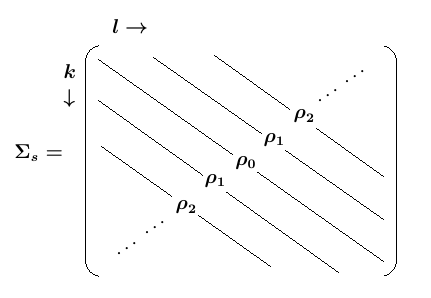
\includegraphics[scale=0.6]{Figures/CovMatWSS.png}
\caption{Structure of the covariance matrix for wide sense stationary signal.}	
\label{fig:CovarianceMat}	
\end{figure}
\noindent i.e., each diagonal is locus of points where $\rho(|k-l|)$ is a constant.\\

\noindent Now from \eqref{l6}, define a scaled version of LMP statistic 

\begin{equation}
\label{l7}
\begin{aligned}
T({\underline{y}}) &\coloneqq\frac{1}{n}{\underline{y}}^T\Sigma_s{\underline{y}}\\
&= \frac{1}{n}\sum\limits_{k=1}^{n}\sum\limits_{l=1}^{n}y_ky_l\rho_{|k-l|}
\end{aligned}
\end{equation}\\ 
Define $\tau = k-l$, then \eqref{l7} simplifies to
 
\begin{equation}
\label{l8}
\begin{aligned}
T({\underline{y}}) &= \frac{1}{n}\sum\limits_{\tau= -(n-1)}^{n-1}\rho_{|\tau|}\sum\limits_{l=1}^{n-\tau}y_ly_{l+\tau}\\
&= \frac{1}{n}\rho_0\sum\limits_{l=1}^{n}y^2_l + \frac{2}{n}\sum\limits_{\tau=1}^{n-1}\rho_{\tau}\sum\limits_{l=1}^{n-\tau}y_ly_{l+\tau}\\
&= \rho_0\hat{\rho_0} + \frac{2}{n}\sum\limits_{\tau=1}^{n-1}\rho_{\tau}\hat{\rho_{\tau}}(n-\tau)
\end{aligned}
\end{equation}\\
where $\hat{\rho_{\tau}}$ is defined by
 
\begin{equation}
\begin{aligned}
\hat{\rho_{\tau}} \coloneqq \frac{1}{n-\tau}\sum\limits_{l=1}^{n-\tau}y_ly_{l+\tau}, \ \ \ \ \tau = 0,1,...,n-1
\end{aligned}
\end{equation}\\ 
Finally, \eqref{l8} can be written as

\begin{equation}
\label{l9}
\begin{aligned}
T({\underline{y}}) = \rho_0\hat{\rho_0} + 2\sum\limits_{\tau=1}^{n-1}\rho_{\tau}\hat{\rho_{\tau}}\left(1-\frac{\tau}{n}\right)
\end{aligned}
\end{equation}\\
The representation of \eqref{l9} leads to the following interpretation of the LMP statistic of \eqref{l7}. For large n, $\hat{\rho_{\tau}}$ is an estimate of the covariance $\mathbbm{E}[Y_lY_{l+\tau}]$. Thus, $T({\underline{y}})$ estimates the covariance structure of the observation and then matches this with the signal covariance sequence.\\
 
\noindent If $n \gg 1$ and $\hat{\rho_{\tau}} \approx \rho_{\tau}$ we can write

\begin{equation}
\label{l10}
T(\underline{y}) =  
\begin{cases}
\rho_0 \ \ \ \ under \ \mathcal{H}_0 \\
\rho_0 + \theta \left(\rho^2_0 + \sum\limits_{\tau = 1}^{n-1}\rho^2_{\tau}\left(1-\frac{\tau}{n}\right)\right) \ \ \ \ under \ \mathcal{H}_1
\end{cases}
\end{equation}\\
We see that $T({\underline{y}})$ discriminates between $\mathcal{H}_0$ and $\mathcal{H}_1$ for $\theta \approx 0$, if the signal is highly correlated(i.e., $\sum\limits_{\tau=1}^{n-1}\rho^2_{\tau}$ is large). 

 

	
\section{Performance Analysis Techniques for general Detectors}

Consider a test of the form
\begin{equation}
\delta_T(y) =  
\begin{cases}
1, &>  \\
\gamma,  \ \ \ \  \mbox{if}~T(y)&= \tau  \\
0. &<
\end{cases}
\end{equation}\\
where {$T: \Gamma \to \R$} is any function. We would like to make statements regarding its detection and false alarm probabilities.\\
\\
Performance of {$\delta_T:$}\\
\begin{equation}
\begin{aligned}
P_F(\delta_T) &= \mathbb{P}_0[T(y)>\tau] + \gamma\mathbb{P}_0[T(y)=\tau]\\
P_M(\delta_T) &= \mathbb{P}_1[T(y)<\tau] + (1-\gamma)\mathbb{P}_1[T(y)=\tau]\\
\end{aligned}	
\end{equation}
\\
In general, if $Y\in \mathbbm{R}^{n}$ and has pdf {$P_0, P_1$} under $\mathcal{H}_0,\mathcal{H}_1$, then\\
\begin{equation}
\label{l11}	
\begin{aligned}
P_F(\delta_T)=\idotsint\limits_{\{y:T(y)>\tau\}}P_0(y)dy
\end{aligned}
\end{equation}
This is not tractable in general.
\subsection{Chernoff Bound Technique}
Since \eqref{l11} is hard to solve for large n, we go on to ask if we could arrive at an approximation for $P_F(\delta_T)$ for large n.\\

\noindent \textbf{\underline{Markov's Inequality:-}} For a random variable $X\geqslant0$, $ a>0$ \\
\begin{equation}
\begin{aligned}
\mathbb{P}[X\geqslant a] \leqslant \frac{\mathbb{E}[X]}{a} 
\end{aligned}
\end{equation}
\textbf{\underline{Proof:-}}

\begin{equation}
\begin{aligned}
\mathbb{P}[X\geqslant a] = \mathbb{E}[\underbrace{\mathbb{I}_{X\geqslant a}}_{\le \frac{X}{a}}]
\leqslant \mathbb{E}
\begin{bmatrix}
\frac{X}{a}
\end{bmatrix}
=\frac{\mathbb{E}[X]}{a}. \ \ \ \ \ \ \blacksquare
\end{aligned}
\end{equation}
 
\noindent We can write,\\
\begin{equation}
\label{l12}
\begin{aligned}
P_F(\delta_T) & \leqslant \mathbb{P}_0[T(Y)\geqslant\tau]\\
&=	\mathbb{P}_0[e^{sT(Y)}\geqslant e^{s\tau}]\\	 	 &\leqslant \mathbb{E}_0[e^{sT(Y)}].e^{-s\tau}\\
&= exp\lbrace-s\tau + \underbrace{log{\mathbb{E}_0[e^{sT(Y)}]}}_{\bydef \mu_{T,0}(s)} \rbrace, \ \ \ \ \forall s\geqslant0 \\
\end{aligned} 	
\end{equation}
where $\mu_{T,0}(s)$ is called the Cumulant Generating Function(C.G.F.) of $T(Y)$ under $\mathcal{H}_0$ at s.\\
Similarly,
\begin{equation}
\label{l13}
\begin{aligned}
P_M(\delta_T) & \leqslant \mathbb{P}_1[T(Y)\leqslant\tau]\\
&=	\mathbb{P}_1[e^{s'T(Y)}\geqslant e^{s'\tau}]\\	 	 &\leqslant exp\lbrace-s'\tau + \underbrace{log{\mathbb{E}_1[e^{s'T(Y)}]}}_{\bydef \mu_{T,1}(s)} \rbrace, \ \ \ \ \forall s'\leqslant0 \\
\end{aligned}
\end{equation}
In general, we would like to choose $s \geqslant 0$, $s' \leqslant 0$ and get the RHS of \eqref{l12} and \eqref{l13} as small as possible.\\
Consider likelihood ratio tests:
\begin{equation}
\begin{aligned}
T(Y)=logL(y)=log\frac{P_1(y)}{P_0(y)}\\
\end{aligned}
\end{equation}
In this case,
\begin{equation}
\begin{aligned}
\mu_{T,1}(s') &= log\mathbb{E}_1[e^{s'logL(y)}]\\
&=log{\mathbb{E}_1[(L(y))^{s'}]}\\
&=log\int (L(y))^{s'}. \frac{P_1(y)}{P_0(y)} dy. P_0(y)\\
&=log\int (L(y))^{1+s'}   P_0(y) dy \\
&=log\mathbb{E}_0 [(L(y))^{1+s'}] \\
&=\mu_{T,0}(1+s')\\
\end{aligned}
\end{equation}\\
Therefore,
\begin{enumerate}\bfseries
\item $P_F(\delta_T)\leqslant {e^{\overbrace{-s\tau + \mu_{T,0}(s)}^{f_1(s)}}}, \ \ \ \ s\geqslant 0$ \\\\$P_M(\delta_T)\leqslant e^{-s'\tau + \mu_{T,0}(1+s')},\ \ \ \ s'\leqslant 0$
\item $P_M(\delta_T)\leqslant e^{\overbrace{(1-s)\tau + \mu_{T,0}(s)}^{f_2(s)}}, \ \ \ \ s\geqslant 1$
\end{enumerate}

\begin{figure}[h]
\centering
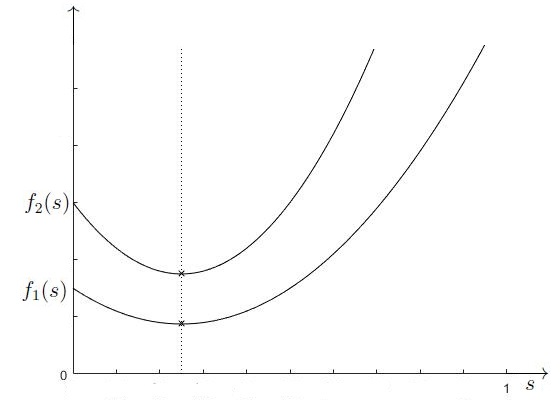
\includegraphics[scale=0.5]{Figures/Convex1}
\caption{Convex function.}
\label{fig:obsspace}
\end{figure}


\noindent \textbf{\underline{FACT:-}} \nonumber $f_1(s)  \bydef \mu_{T,0}(s)-s\tau \text{ and } f_2(s) \text{ are CONVEX functions of s, refer Figure \ref{fig:obsspace}.}$\\
\\
\text{For a convex function,}
\begin{center}
$\forall x,y, \forall \lambda \in [0,1].$\\
$f_1(\lambda x + (1- \lambda)y)\le \lambda f_1(x)+(1-\lambda)f_1(y)$\\
\end{center}

	
\end{document}